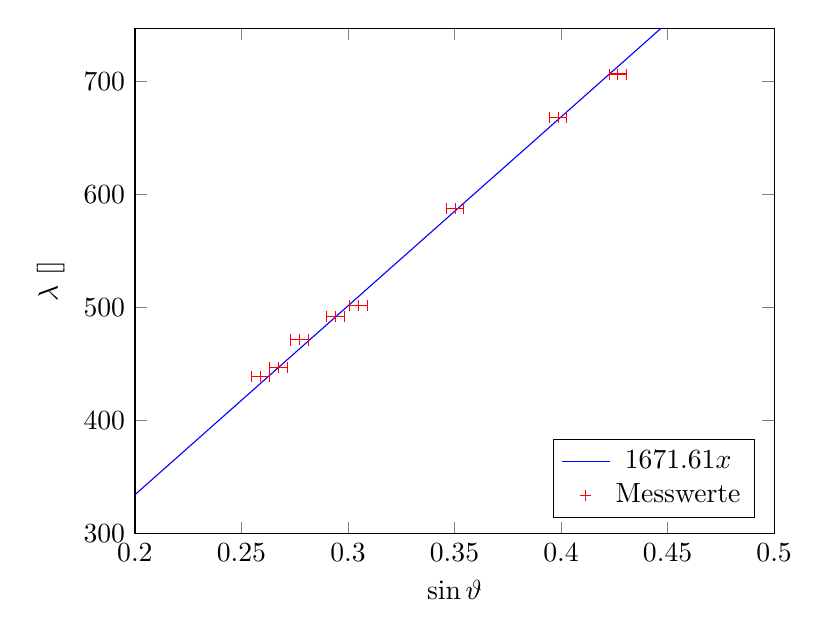
\begin{tikzpicture}
\begin{axis}[xmin = 0.2, ymin = 300, xmax = .5,
	legend pos = south east, width = .8\textwidth, height = 8cm,
	xlabel = $ \sin\vartheta $,
	ylabel = {$ \lambda $ [\si{\nano\meter}]}]
	
	\addplot+[no marks, ] {1671.61*x};
	\addplot+[mark = +,only marks, error bars/.cd, x dir = both, x explicit,] table[x=x,y=y, x error = xerr] {
y	x	xerr
438.8	0.2588190451	0.0042146465
447.1	0.2672383761	0.004204631
471.3	0.2773146533	0.0041921899
492.2	0.2940403252	0.0041704338
501.5	0.304864299	0.0041556106
587.5	0.3502073813	0.0040870034
667.8	0.3987490689	0.0040014294
706.5	0.4265687399	0.0039464301
};
\legend{{$ \num{1671.61}x $}, Messwerte}
\end{axis}
\end{tikzpicture}